
\chapter{Introduction}
\label{ch:Introduccion}

\section{Context}
Parkinson’s disease is a chronic and progressive movement disorder due to the malfuction and death of neurons in the brain. Some of these neurons produce dopamina, a chemical that sends messages to the part of the brain that controls movement and coordination. Thus, as Parkinson’s disease progresses,  the amount of dopamine produced in the brain decreases, leaving the person unable to control movement normally \cite{pdf}.

The disease must be diagnosed by an experienced neurologist. There are no tests that clearly identify the disease, but brain scans and blood test are sometimes used to rule out disorders that could give similar symptoms. 
One of the main concerns of people with PD is the fear of falling. First motor symptoms in this disease, like rigidity (stiffness  of the limbs and trunk), bradykinesia (slowness of movement) and postural changes, contribute to  risk of falling. Difficulties in the adaptation of neck and trunk cause  postural instability, which, in turn, increase the possibility of suffering a fall.

The center of body mass of a person is situated below the navel and the legs work as a support base. In PD it is common that the center of  mass goes out of support base. This fact causes losses of equilibrium in activities such as waking up, bending, spinning  around quickly or walking. Also, falls can occur due to a damage in postural reflexes (a series of complex movements that we carry out in an automatic way in order to maintain the equilibrium when we get up and walk), postural changes (tendency to lean forward using short, quick steps and reduced arm movement) and freezing (inability to step that delays gait initiation or interrupts ongoing gait). Research in this field is of vital importance to contribute to the improvement of knowledge about the disease. Scientific research can be the base for  field applications that help to improve the people life with PD. \cite{ParkinsonDisease}\cite{pdf}

With this Project, we aim  to contiue the research line initiated by Dr. Alberto Olivares, member of the SIPBA (Signal Processing and Biomedical Applications) research group of the Department of Signal Theory, Telematics and Communications of the University of Granada, Spain, and Prof. Dr. Med. Kai Bötzel, head of the Motion Analysis and Deep Brain Stimulation Laboratory of the Department of Neurology of the Klinikum Grosshadern based in Munich, Germany. In his dissertation ,Dr. Olivares explains in his Ph.D. thesis \cite{A.Olivares2013} different signal processing techniques to analyze information from inertial sensors to monitor human body motion.
Specifically, our work will be focused on signal processing of data gathered  by a force plate and a wearable motion analysis system based on inertial sensors . Nevertheless, this master thesis is part of a broader project which has many different layers (instrumentation, data gathering, firmware, signal processing) in which other people have been working during the last 5 years .

 IMAGE 

\section{Motivation}
Parkinson’s disease is the second most common neurodegenerative disorder, it is extended globally and affects as much to men as to women. PD is more common among the population over 60 years old. . It is estimated that seven  to ten million people worldwide are living with Parkinson’s disease. To this date, there is no cure to PD, so all efforts are focused on improving or prolonging the functionality of the patient for as long as possible. Therefore, it’s an incentive to work in this field. \cite{ParkinsonDisease}\cite{pdf}

Furthermore, Intel and Michael J.Fox Fundation have rencently teamed up to create a sensor technology and analytics platforms for Parkinson’s treatment and monitoring. Fox Foundation CEO Todd Sherer told Fast Company. "Parkinson’s is a motor disorder for the most part, with slowness of movement, tremors, falls, problems sleeping, and many disease symptoms. The way it is measured right now requires episodic periodic visits to a neurologist, who puts patients through fairly subjective and coarse clinical tests, there are many 1-2-3-4 scales. What we need to advance is research that is a much more consistent and objective measure of the disease. People live with Parkinson’s 24 hours a day, 7 days a week, not just when they're in the doctor’s office."\cite{IntelAndMjf}

The goal is tracking the  symptoms and progress of Parkinson’s disease day by day, and using this information to research on the disease in depth.

\begin{figure}[H]
	\centering
	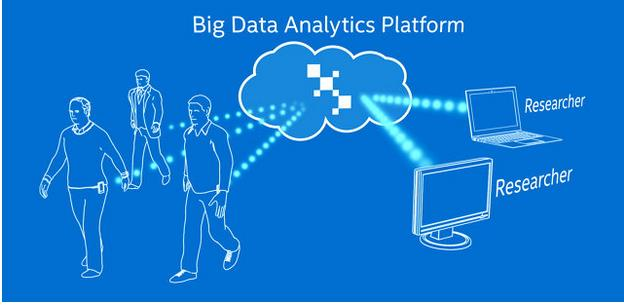
\epsfig{file=imagenes/IntelAndMjf, width=7cm}
	\caption{Illustration of sensors distribution thought up by Intel and Mjf.\cite{IntelAndMjf}}
	\label{fig:arte1}
\end{figure}

Diane Bryant, senior vice president of Intel's Data Center Group, said in a release \cite{IntelAndMjf}.
''Emerging technologies can not only create a new paradigm for measurement of Parkinson's, but as more data is made available to the medical community, it may also point to currently unidentified features of the disease that could lead to new areas of research'' .

\section{Goals}

The main goal of this project is to perform a thorough analysis of Anticipatory Postural Adjustments (referred to as APA in the remainder of this document) of both healthy subjects and PD patients. APAs can be used to characterize step initiation deficits in subjects with PD and also as a differentiating factor which may help early diagnosis of the disease.

To this purpose, we will make use of a database gathered by the medical team in Munich. The database contains both data from a force plate and inertial sensors. The patients wear the motion monitoring system containing the inertial sensors while they step on and down the force plate.

Once the measurements are made, the main objective is to determine whether it is possible to use inertial sensors to extract the information provided by the force plate. That is, we will evaluate the correlation between inertial sensor measurements and the force plate measurements in order to study the feasibility of the wearable device to study APAs in an ambulatory way. 

Additionally, we will try observing if APAs are homogeneus in healthy subjects and the differences with  PD patients. If that is the case, we would be able to build a classifier which is able to distinguish healthy subjects from PD patients based on the data measured by the wearable device and/or the force plate.

In a nutshell, the ultimate goal is to determine whether doctors can substitute force plates (which strongly limit the range of action of the patients) by the inertial wearable system (which allows ambulatory).


\section{Project structure}

\section{State of the art}

We will start studying some current devices used for body monotoring as well as their benefits.

Later we will search the methods and experimental procedures used in several studies to analyse of Anticipatory Postural Adjustments in diferents cases, as well as their applications.

Finally, we will speak about the commons calibration techniques, signal processing and classification.


\subsection{Instrumentation}

There are several  device types used to measure APAs. The most importants are: electromyograph, force platform, inertial sensors and devices based on cameras. 

Electromyography (EMG) is a technique that gives us information about the electrical activity produced by skeletal muscles (See figure [1]). The electromyograph can detect  the electrical activity due a electrical potencial difference generated by muscle cells. It’s very useful to analyse posture, locate injuries like muscle paralysis and the place where they are. \cite{Marcio2010} \cite{Instr1}. 


So far, most of realised studies have included like measurement devices, among other things, a platform sensitive to force and pressure. However, the cost and complex of APAs measurement with a traditional movement analysis, using force platform and EMG System limit their applications in the  clinical practice. Therefore, small inertial sensors are used recently because they are cheaper and more portables. But even so, we have used this platform, considering the posibility to ignore it in the future. \cite{Mancini2009} \cite{Vennila2011}.

Devices based in commonly used inertial sensors are IMU (inertial measurement unit), It’s a electronic device that measures and reports about speed, orientation and gravity force of equipment, using the combination of accelerometers and gyroscopes.
In addition, you can combinate it with magnetometers, but in this case, the device is called MIMO. Some current MIMO are: 3DN-GX4-45 \cite{Instr2},  xsens-mvn \cite{Instr3} y mvn-biomech \cite{Instr4}, all of them use Microelectromechanical Systems (MEMS).

\begin{figure}[H]
	\centering
	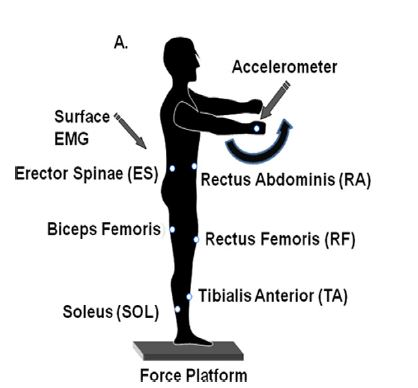
\epsfig{file=imagenes/Captura, width=7cm}
	\caption{EMG, accelerometers y platform \cite{Gay2011}.}
	\label{fig:arte1}
\end{figure}

There are  infrared-reflective markers that give us a complex posture measurement. They are attached  to the body and can provide information about postural strategies, so we can know if the subject uses the ankle strategy or the hip strategy. For example, figure [2] shows the System.

\begin{figure}[H]
	\centering
	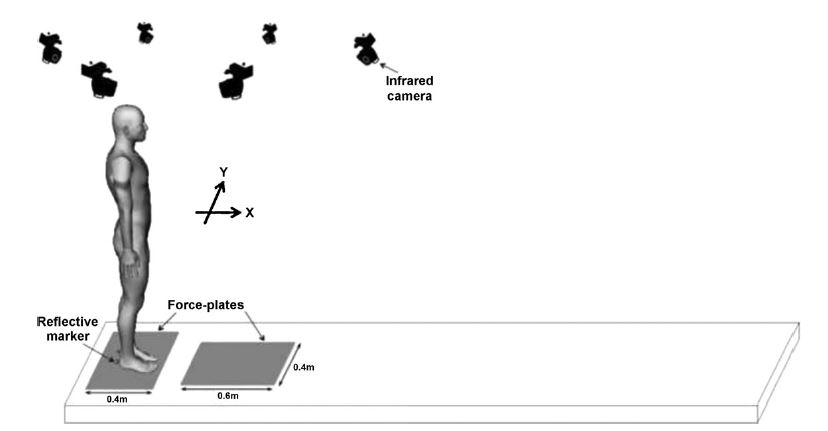
\epsfig{file=imagenes/Captura2, width=7cm}
	\caption{Illustration of the experiment with infrared-reflective markers\cite{Teddy2013}.}
	\label{fig:arte2}
\end{figure}

As mentioned previously, it's possible to use sensors based in cameras that generally are part of a optical System of movement capture such  as Kinect. \cite{Instr5}.


\subsection{Methods and procedure}

So far, a lot of studies about Anticipatory Postural Adjustments are been done, mainly in the  last six years. The finality of the most of this research is be able to deepen knowledge about the posture prior to step initation, and whether there are postural patterns and conditions on which they depend.

If we analyse the state of the art of APAs, we can find that first investigations tried to verify whether APAs are associated to voluntaries movements or no,  this hypothesis was confirmed and the conclusion was it’s more probable that the adjustments don’t appear if step initation isn’t planned. It’s essential for balance control in gait initation because we can use this knowledge to prevent the falls in some people with movement difficults.\cite{Mcllroy1993}\cite{Yiou2012}\cite{Teddy2013}\cite{Bouisset2008}\cite{Neeta2014}

After of this, researchers tried to explain the influence of other variables, such as several exercices that estimulate differents muscles and the reaction of others\cite{Gay2011}; the age influence for generating postural patterns \cite{Bleuse2006} \cite{Estelle2008}; the signal type that initiates the movement ( visual or auditory) due that it affect initial posture \cite{Mcllroy1993}\cite{Antonia2009}\cite{Vicent1999}\cite{Tard2013}; the fear to fall because it can do that patients adopt differents postures[26]; neurodegenerative disease, like Parkinson and Multiple Sclerosis\cite{Mancini2009}\cite{Jebb2008}\cite{Chris2005}\cite{Hall2013}, or cerebral palsy, like hemiplegia and diplegia, \cite{Hall2013}, generate differences in the APAs too.

All these studies are very important in medical applications. For example, As mentioned previously, there are diseases that affect central nervous System, so it affects  the mobility too. Then, it causes falls in many occasions, therefore  the people that suffer the fall have fear of fall again. The fact that fear of fall causes variations in the APAs doing people  fall again, can help us to prevent them.

\subsection{Data Analysis}

In the last years, it has carried out a lot of Works about  calibration of accelerometers and gyroscopes, although the most of them show little variation with others studies done before. One of the most important research  \cite{Kian2011}explains one form to do the calibration putting the acceleromentes in six differents positions and applying  simple algebraic algorithms to the obtained data. The gyroscope is calibrated of different form, using a process based in a known rotation. Also, there are others with the same fundament.

There are other methods that try to be more precise, increasing the number of positions where we record the data \cite{Camps2009}. Also, there are others type of calibration techniques like algorithms based in basic algebraic calculation or in FIR filters. \cite{A.Olivares2013}

As for estimation of orientation for human-body monitoring, if we study the works done so far, we can see that almost all  use a Kalman filter. However, the result with lower signals isn’t very accurate.\cite{A.Olivares2013}

Finally, we will analysis the state of the art of movement recognition in human and classifiers. Quickly, we can see a lot of information about classification because there are a lot of articles and books about this. However, there are others type of studies, which we focus on  it \cite{Banos2012}, that explains methods for human activity recognition based on a sensor weighting hierarchical classifier. This study shows different classification forms that we can use depending on the activities, such as walking or running.

